\epigraph{``Of course it is happening inside your head, Harry, but why on earth should that mean it is not real?"}{Albus Dumbledore}

\section{Root Mean Squared Error}
\begin{figure}[H]
    \centering
    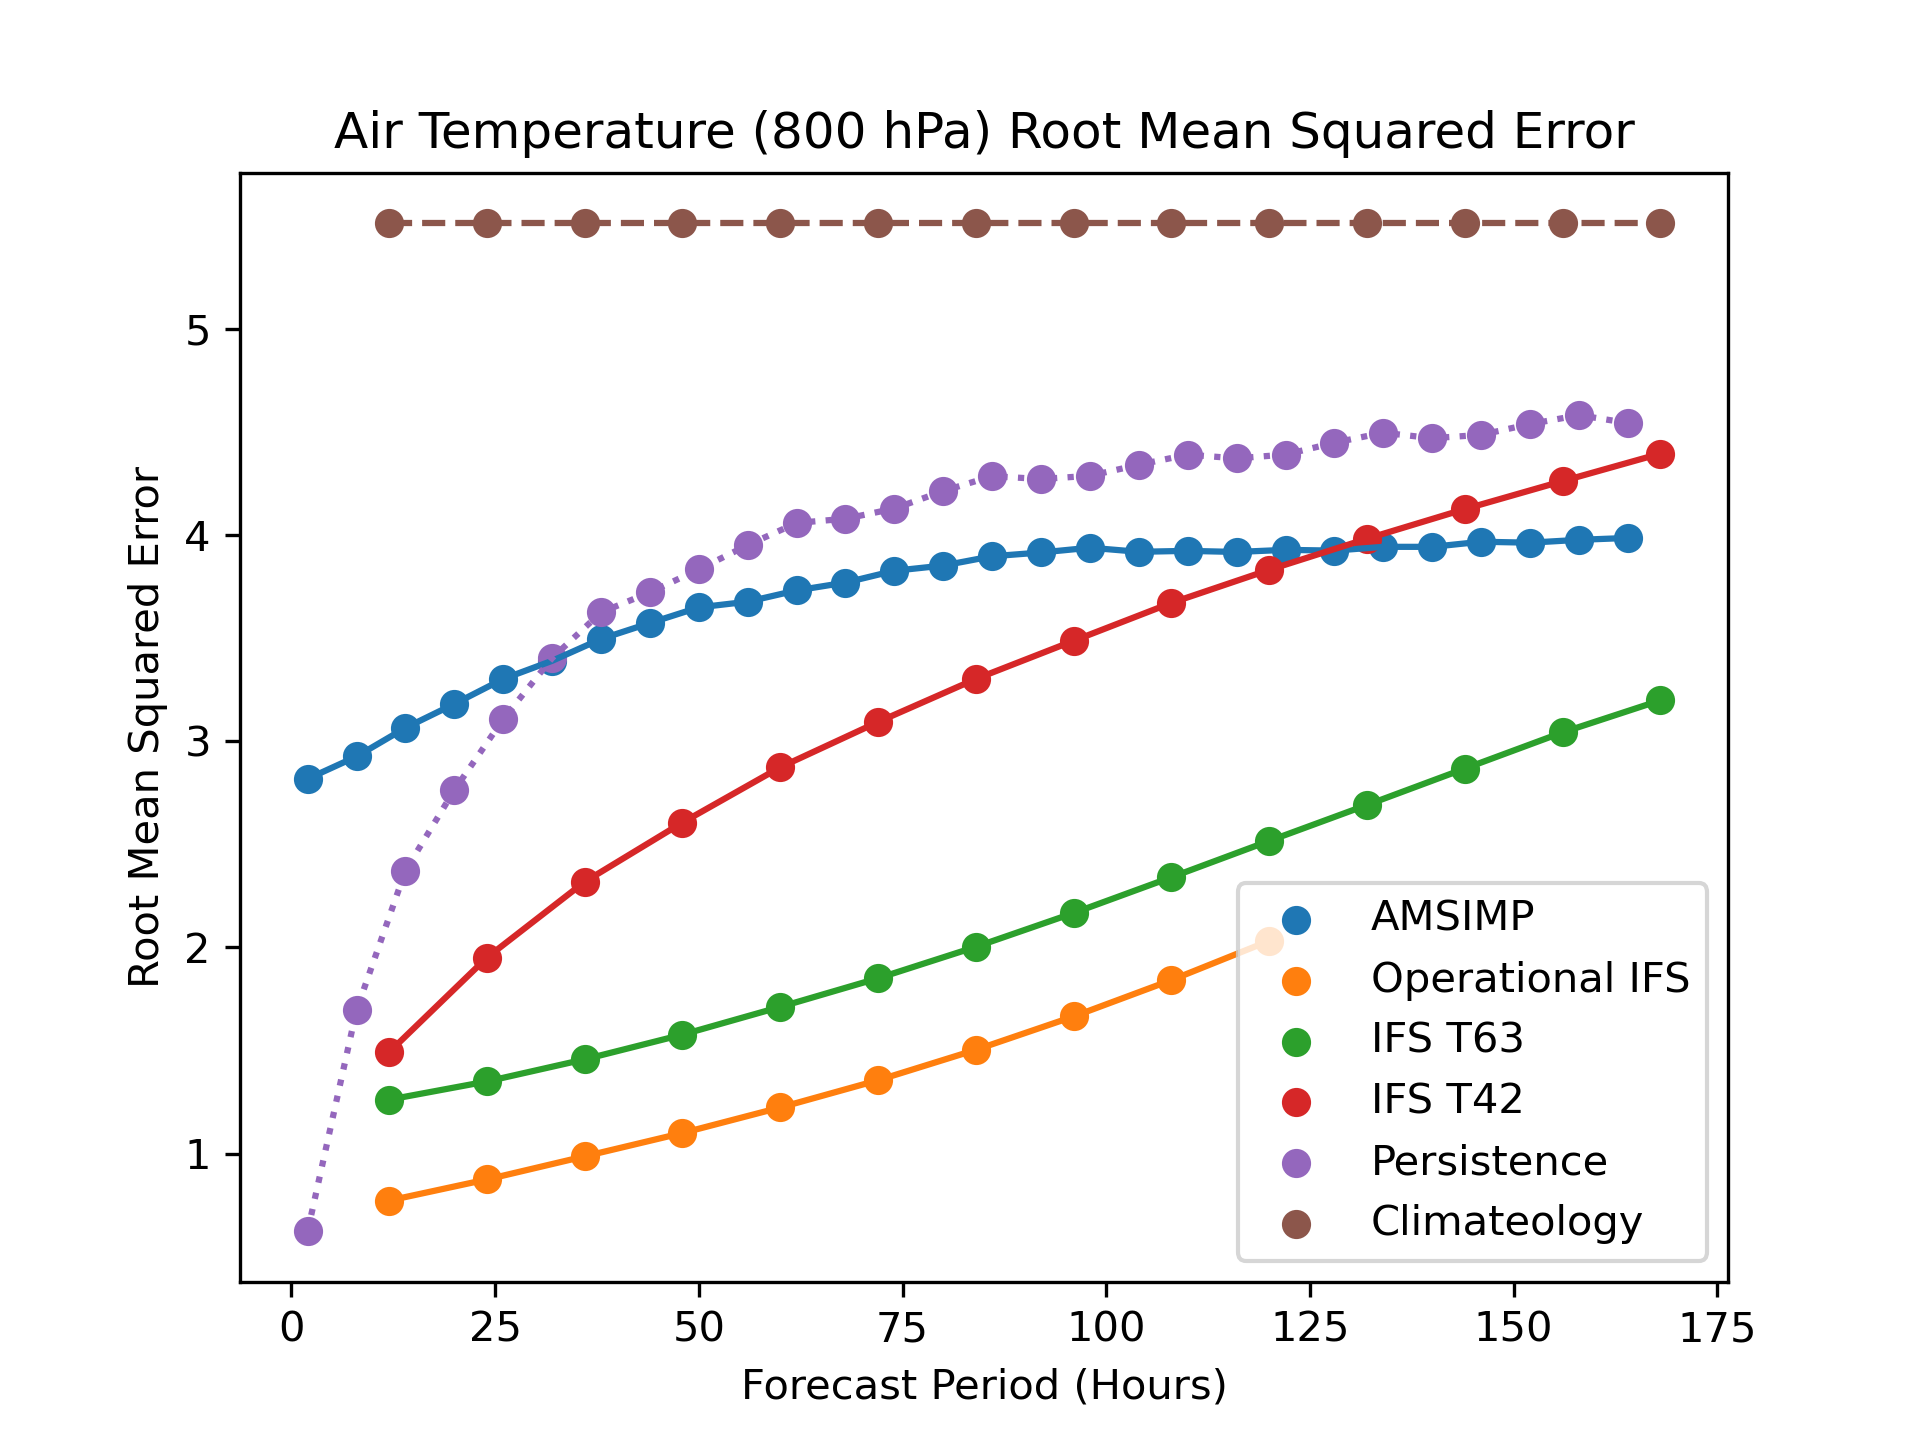
\includegraphics[width=.7\linewidth]{Plots/Results/Temperature/root_mean_squared_error.png}
    \caption{Air Temperature at 850 hPa}
\end{figure}

\begin{figure}[H]
    \centering
    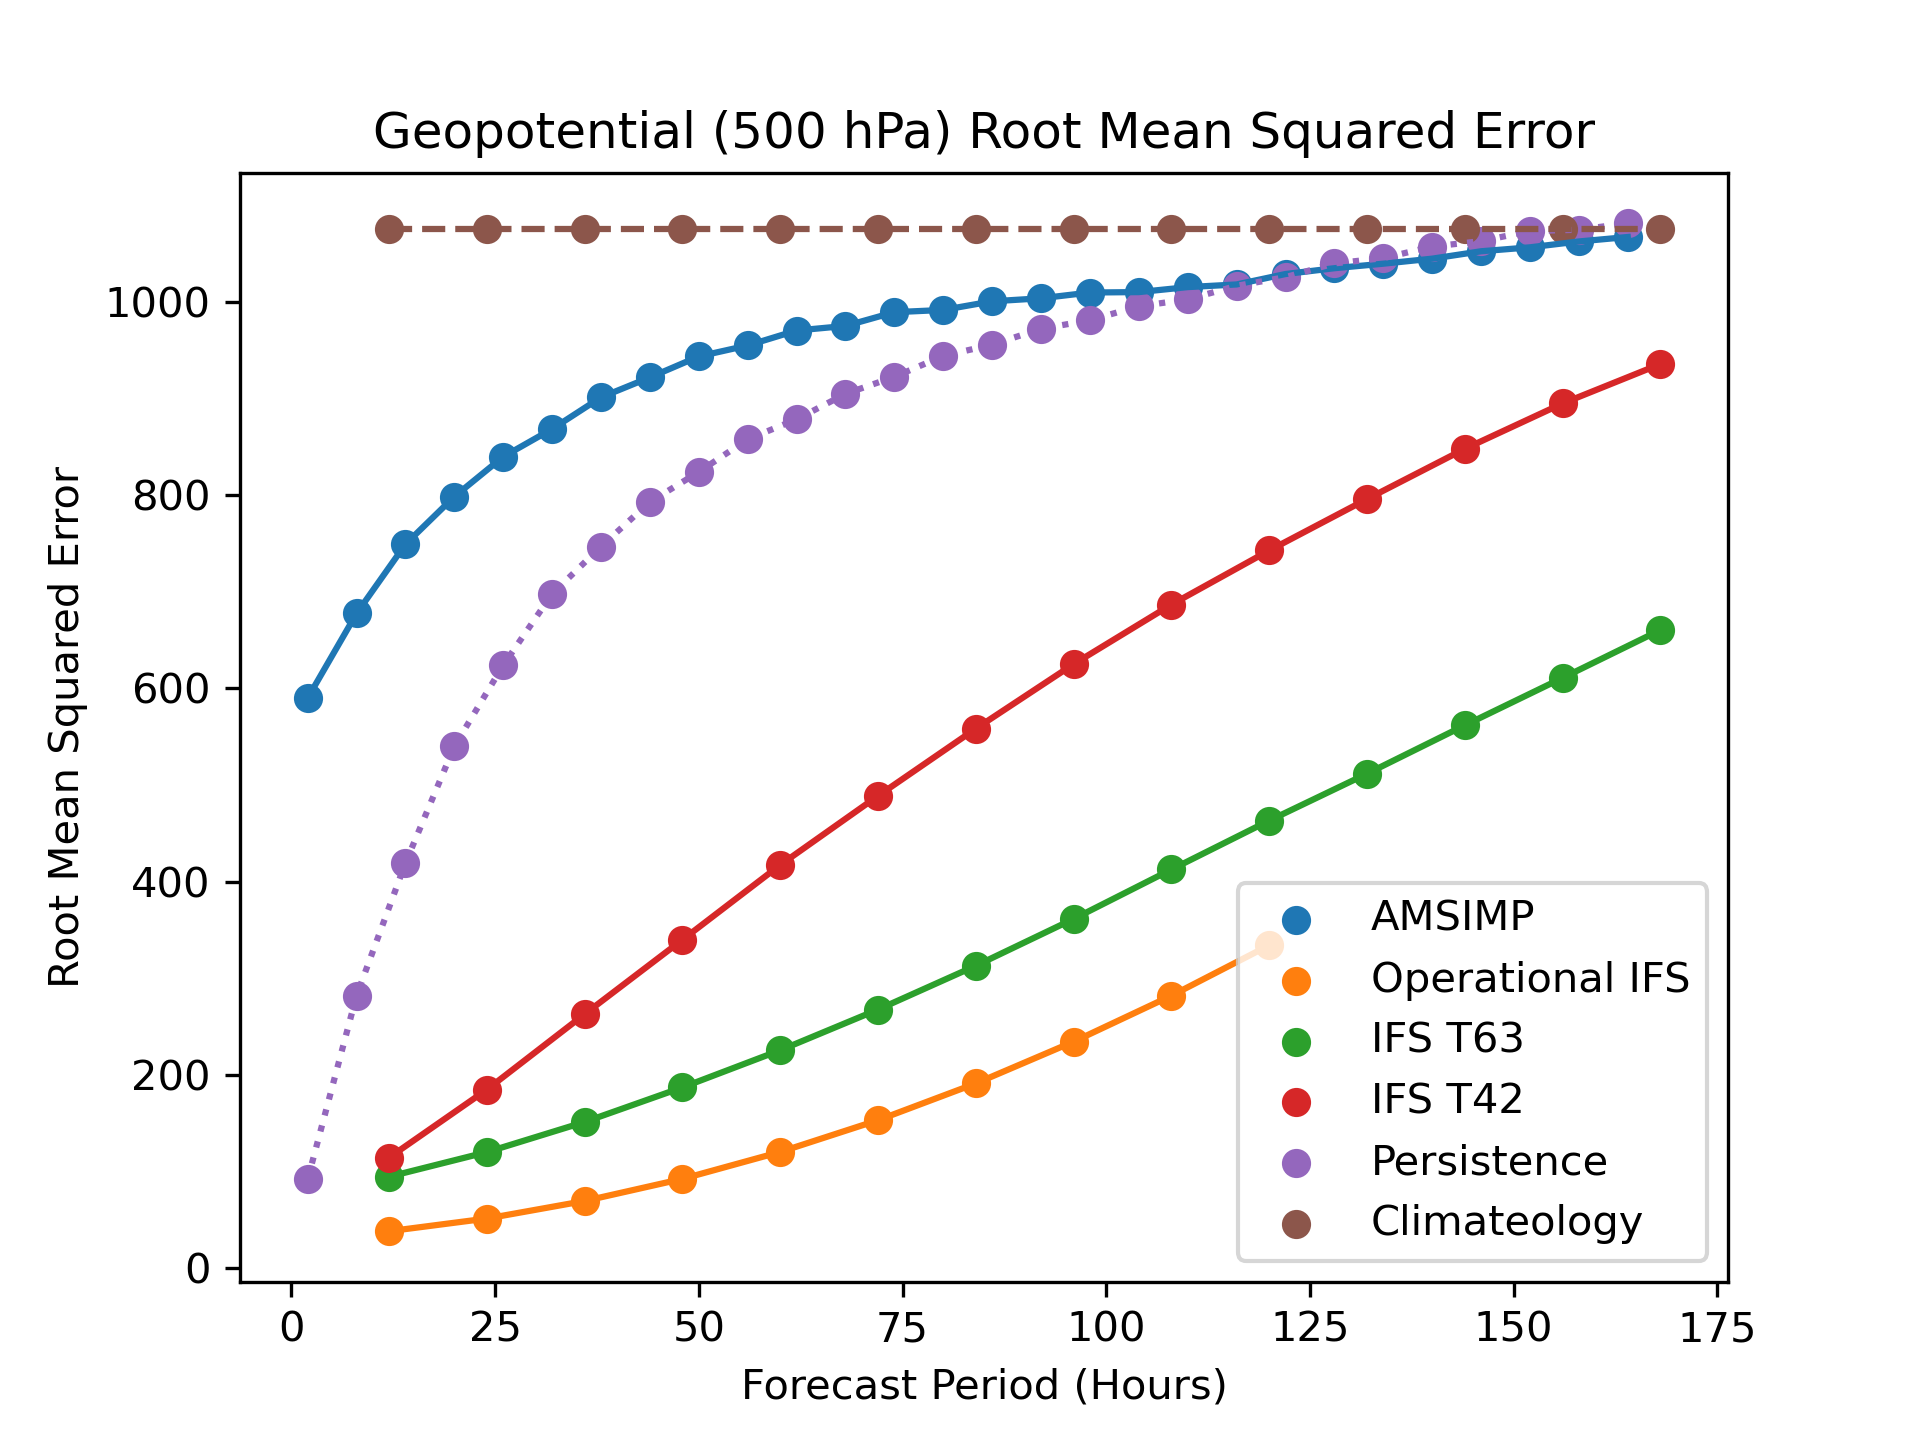
\includegraphics[width=.7\linewidth]{Plots/Results/Geopotential/root_mean_squared_error.png}
    \caption{Geopotential at 500 hPa}
\end{figure}

\section{Mean Absolute Scaled Error}
\begin{figure}[H]
    \centering
    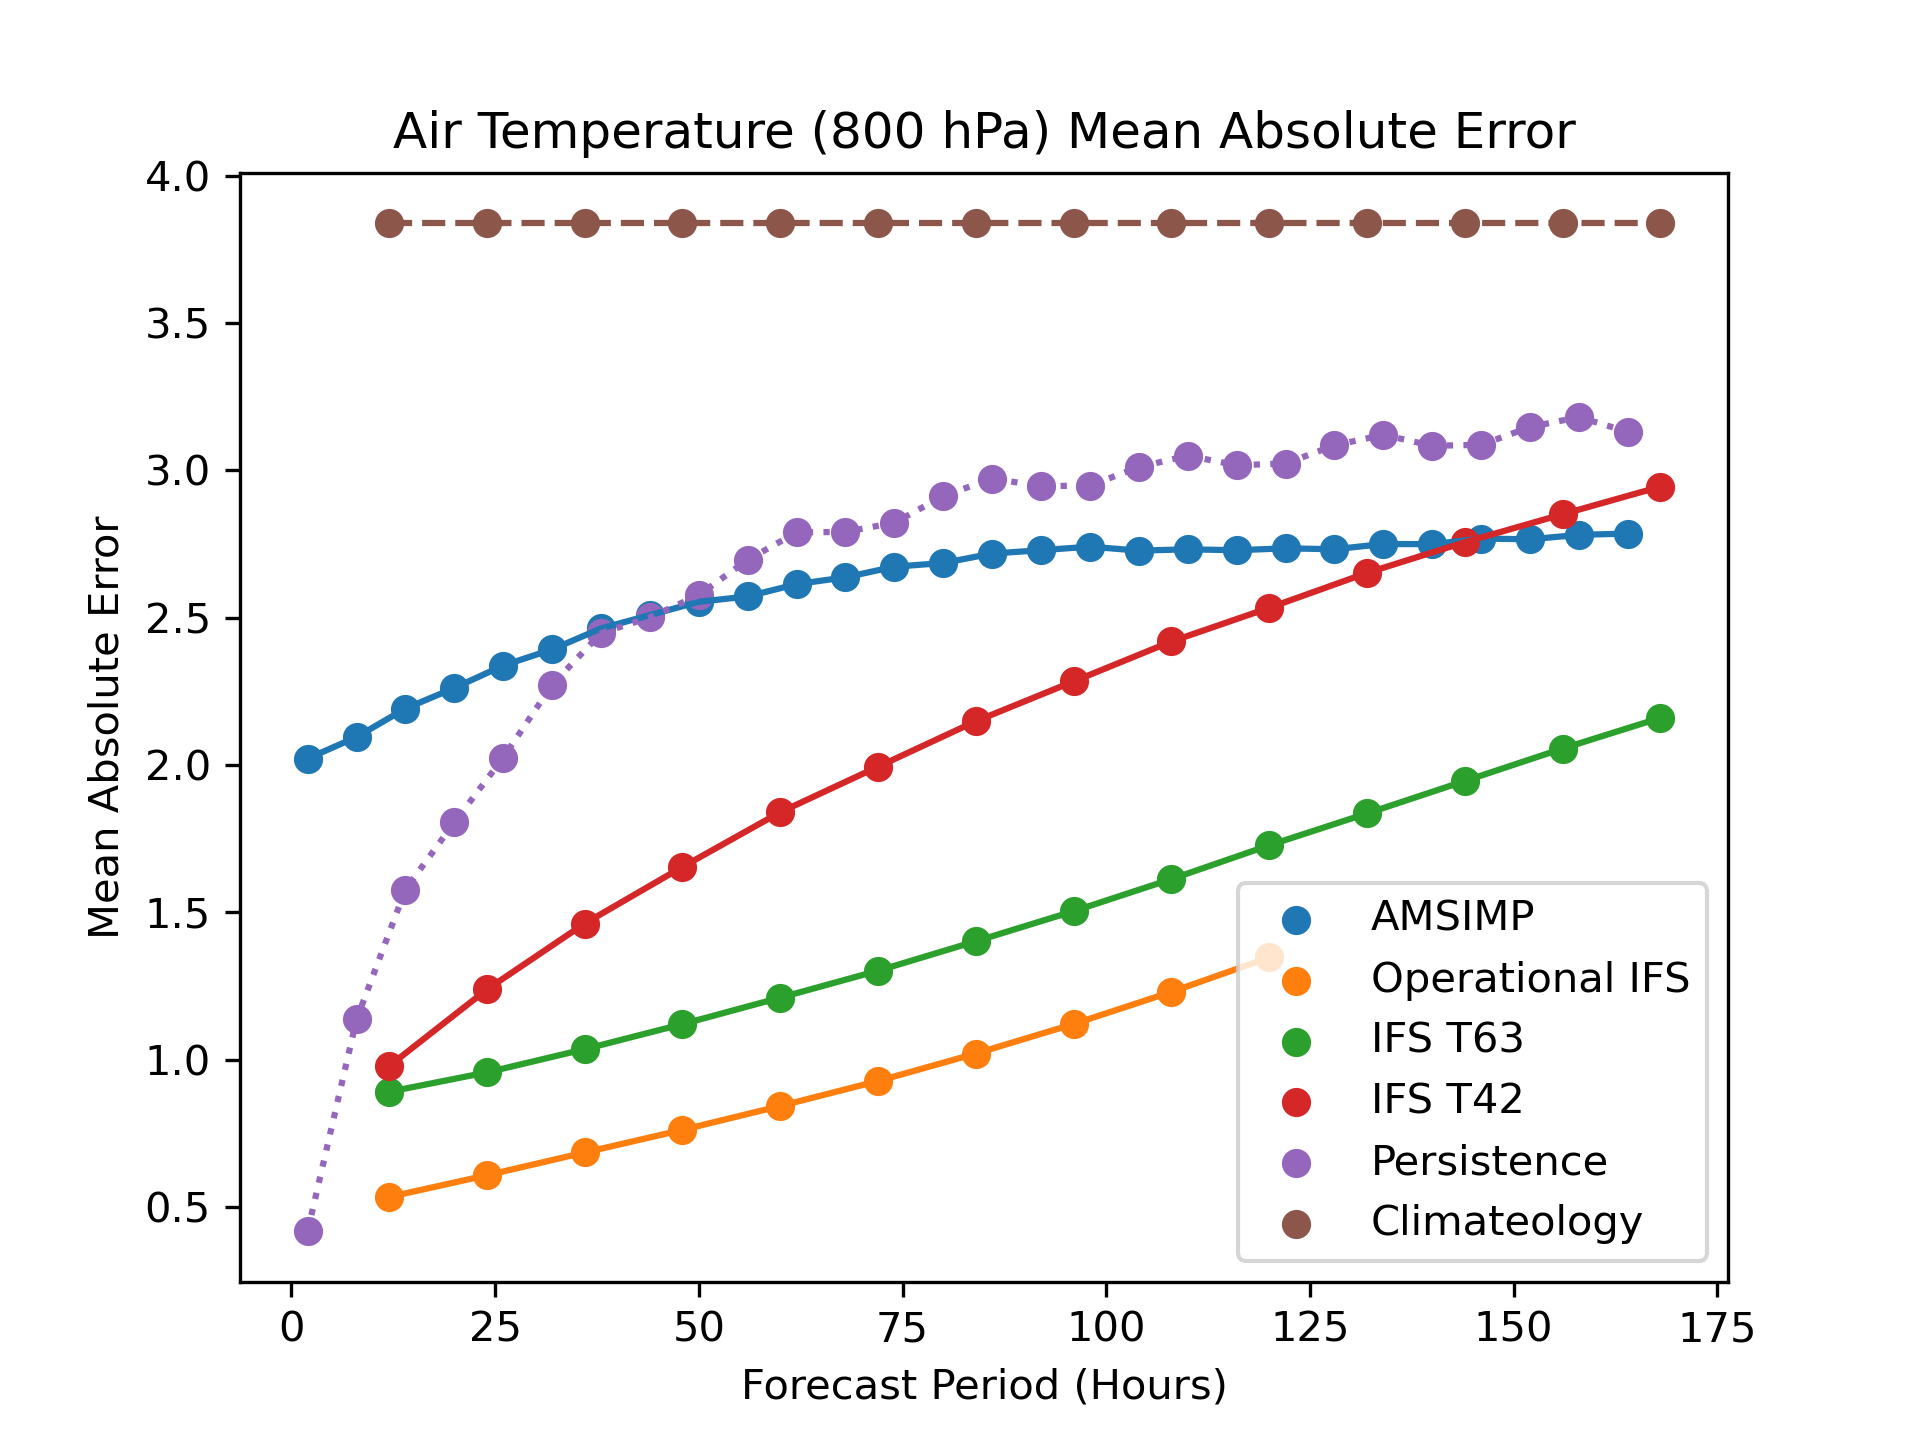
\includegraphics[width=.7\linewidth]{Plots/Results/Temperature/mean_absolute_error.png}
    \caption{Air Temperature at 850 hPa}
\end{figure}

\begin{figure}[H]
    \centering
    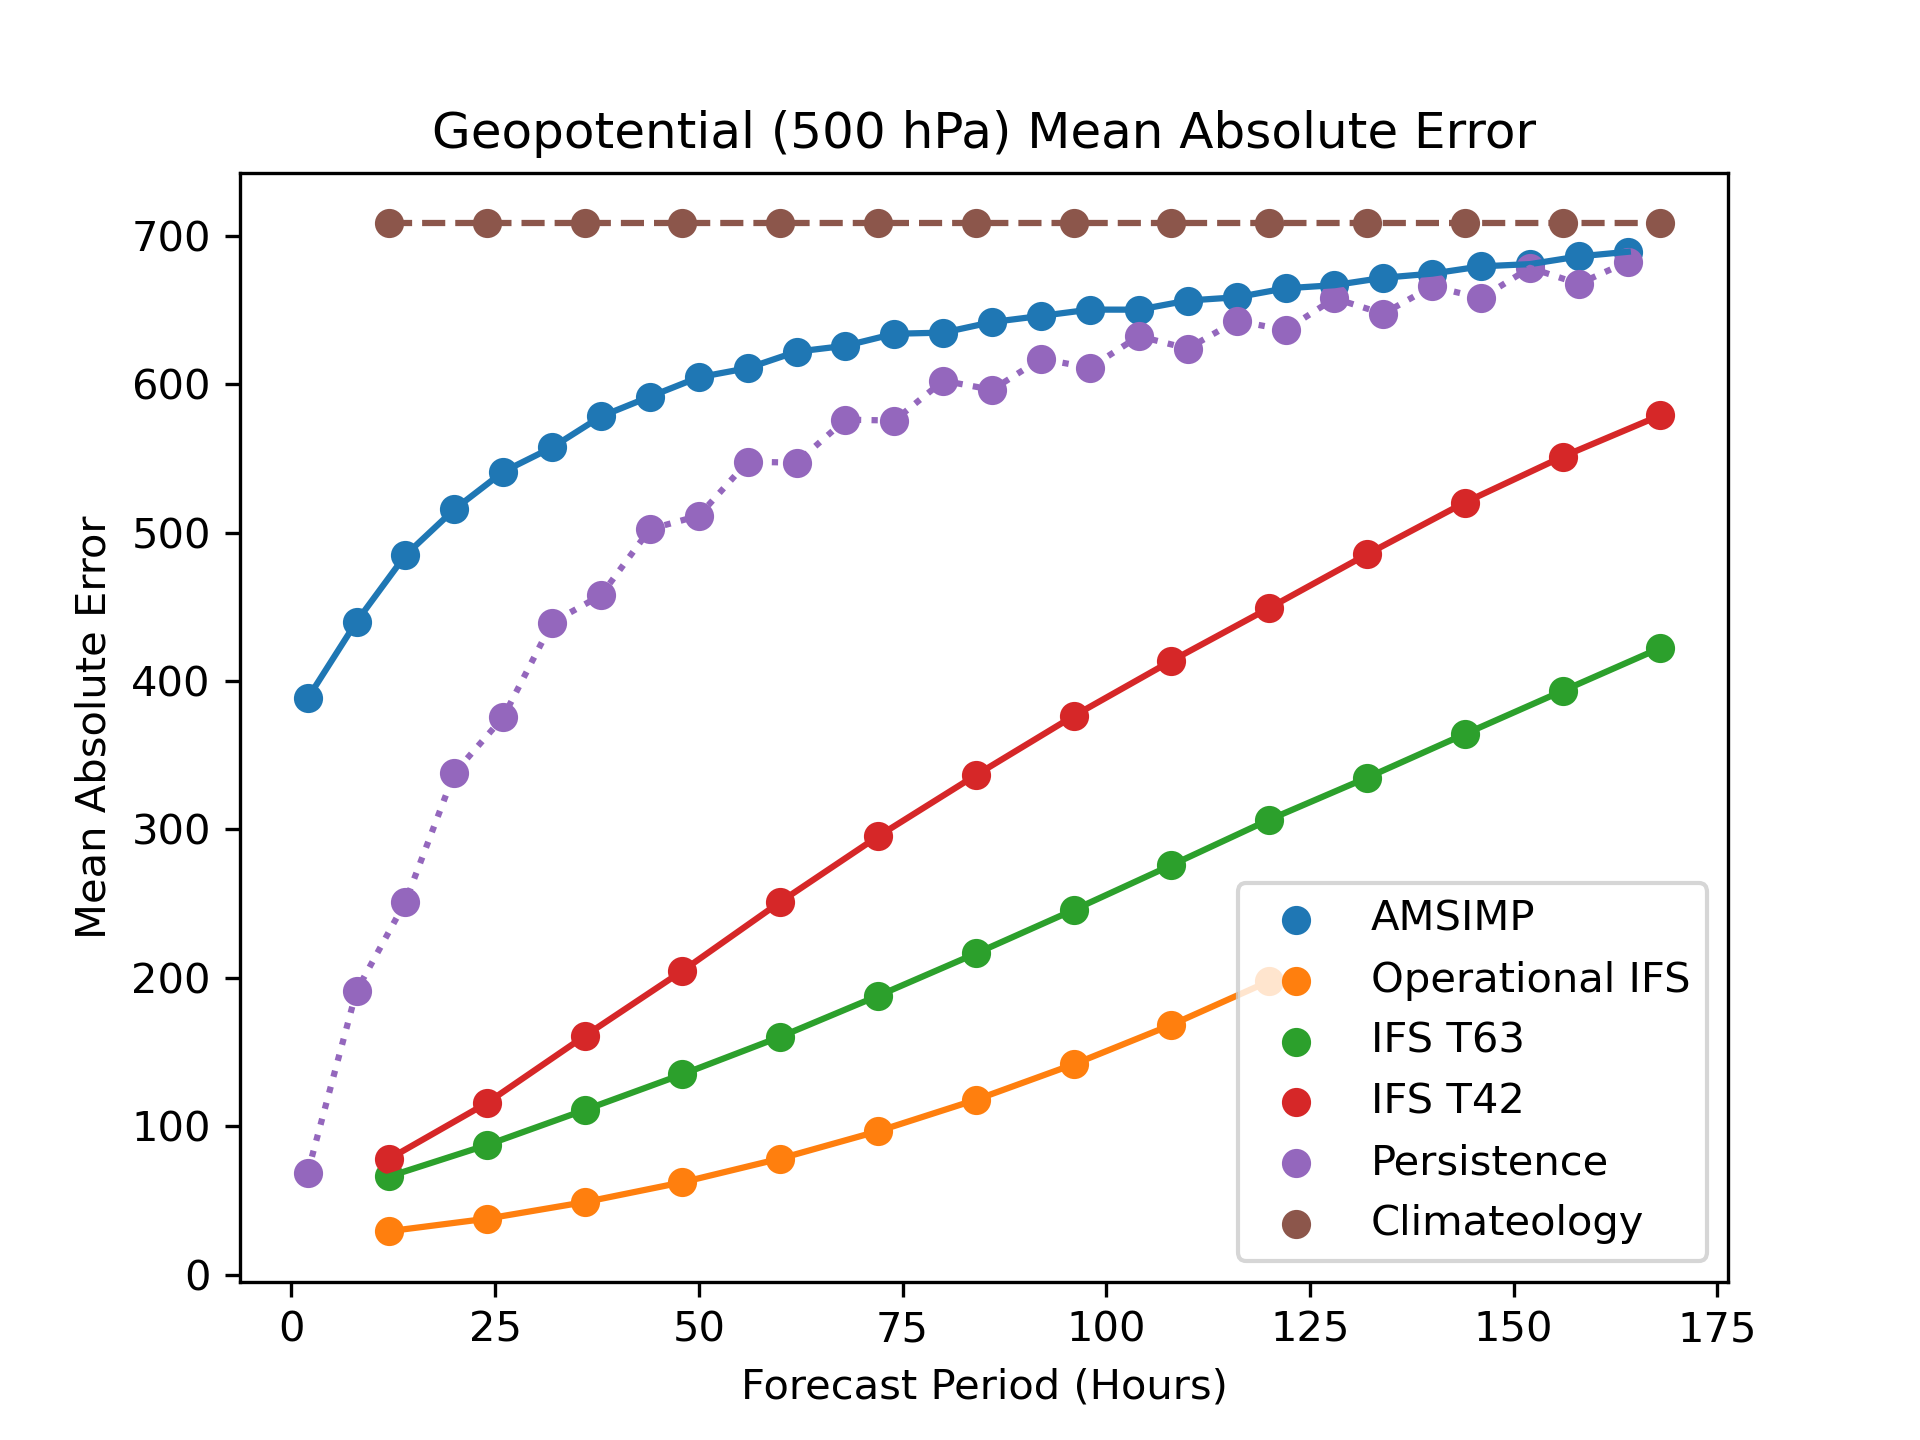
\includegraphics[width=.7\linewidth]{Plots/Results/Geopotential/mean_absolute_error.png}
    \caption{Geopotential at 500 hPa}
\end{figure}

\section{Anomaly Correlation Coefficient}
\begin{figure}[H]
    \centering
    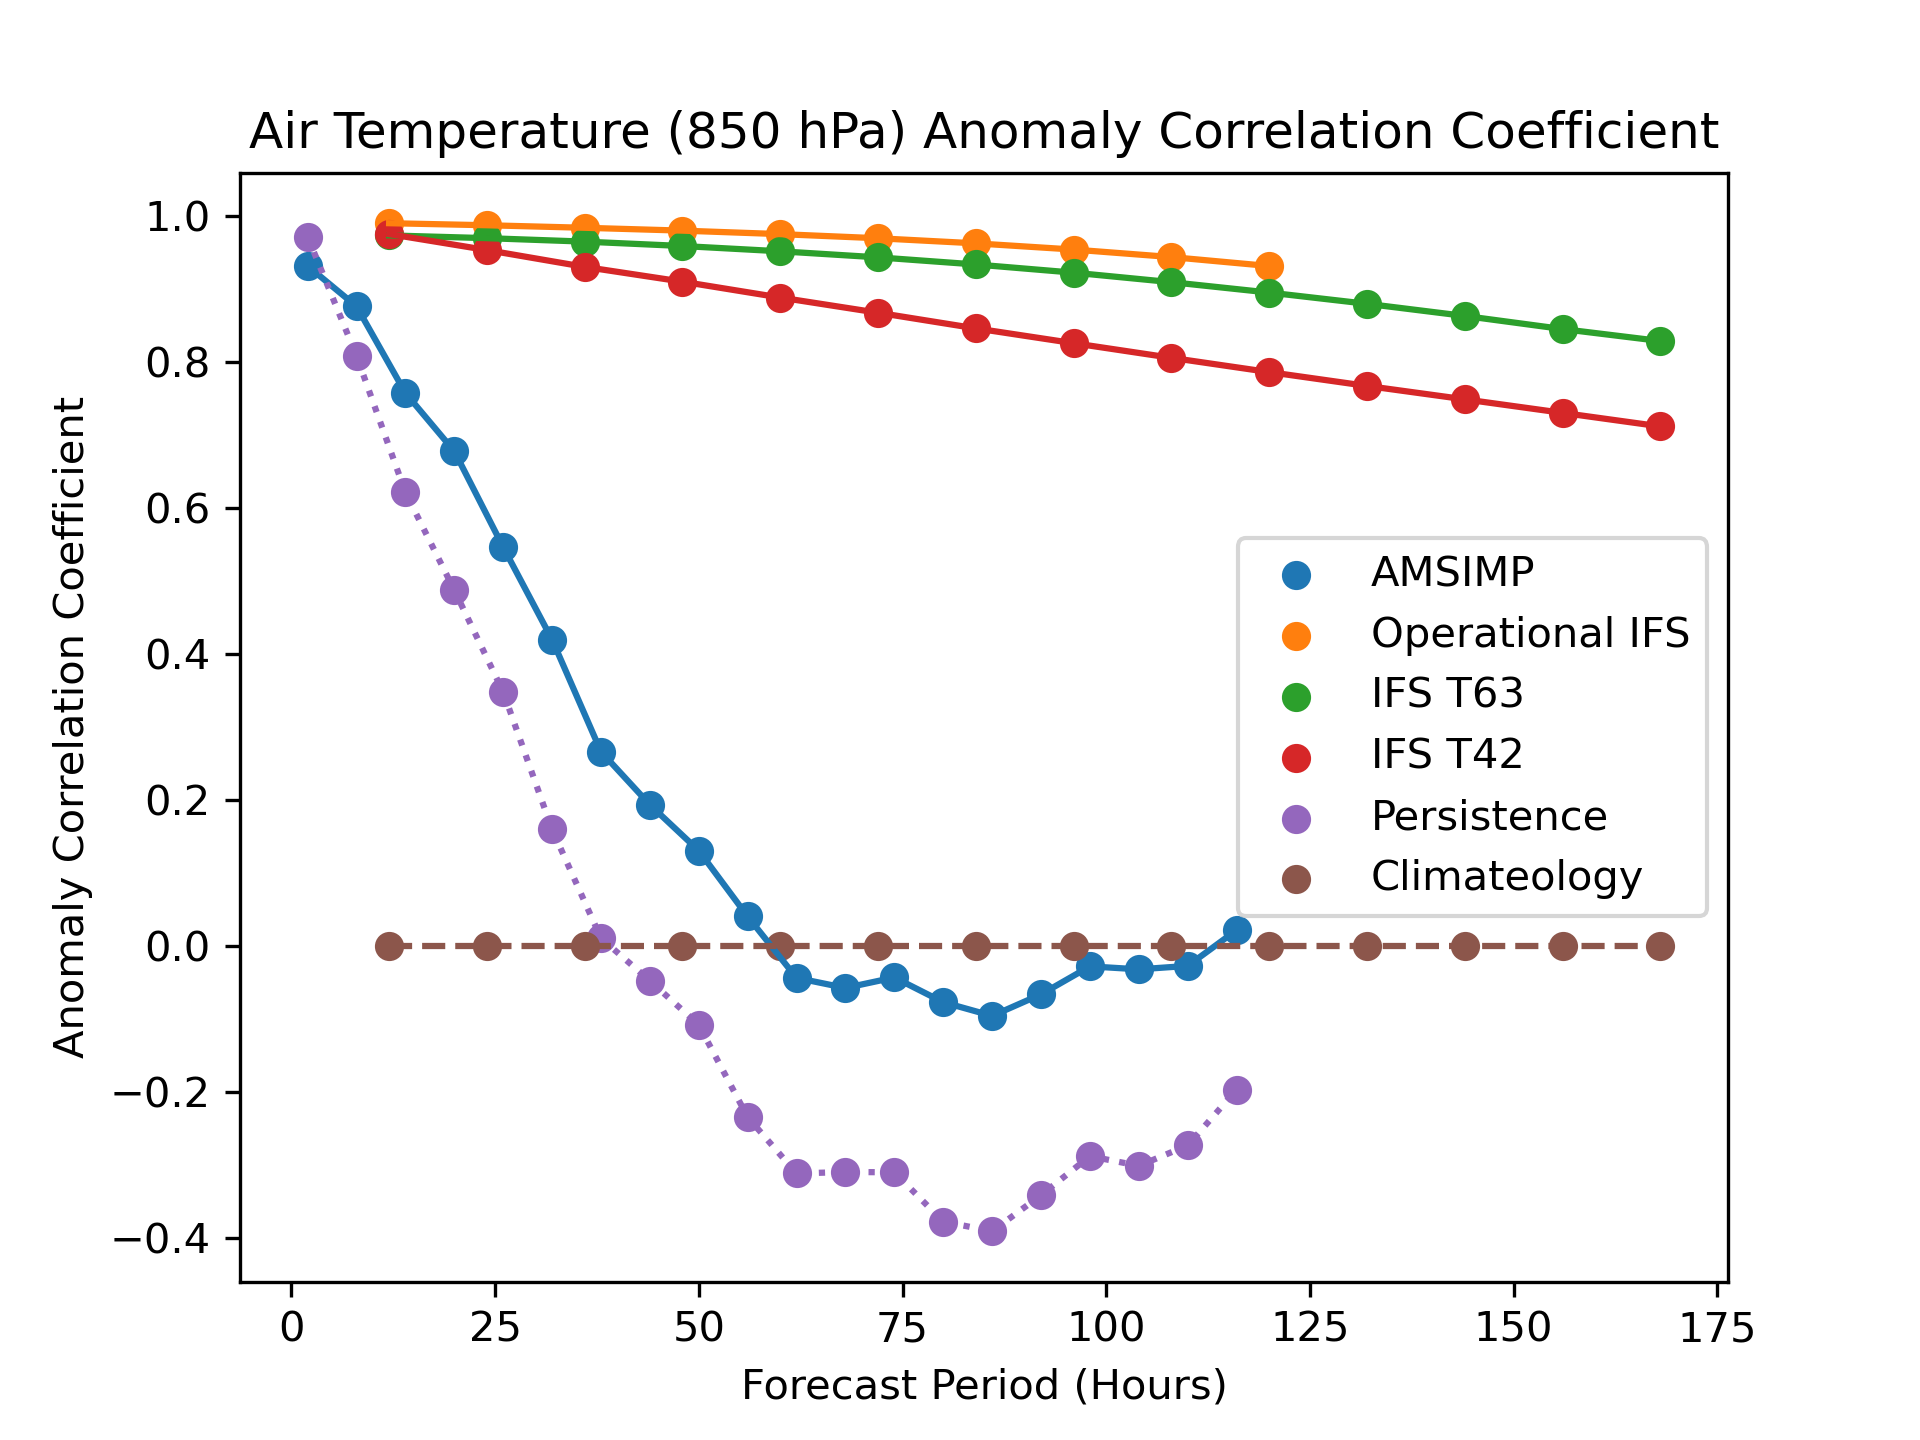
\includegraphics[width=.7\linewidth]{Plots/Results/Temperature/anomaly_correlation_coefficient.png}
    \caption{Air Temperature at 850 hPa}
\end{figure}

\begin{figure}[H]
    \centering
    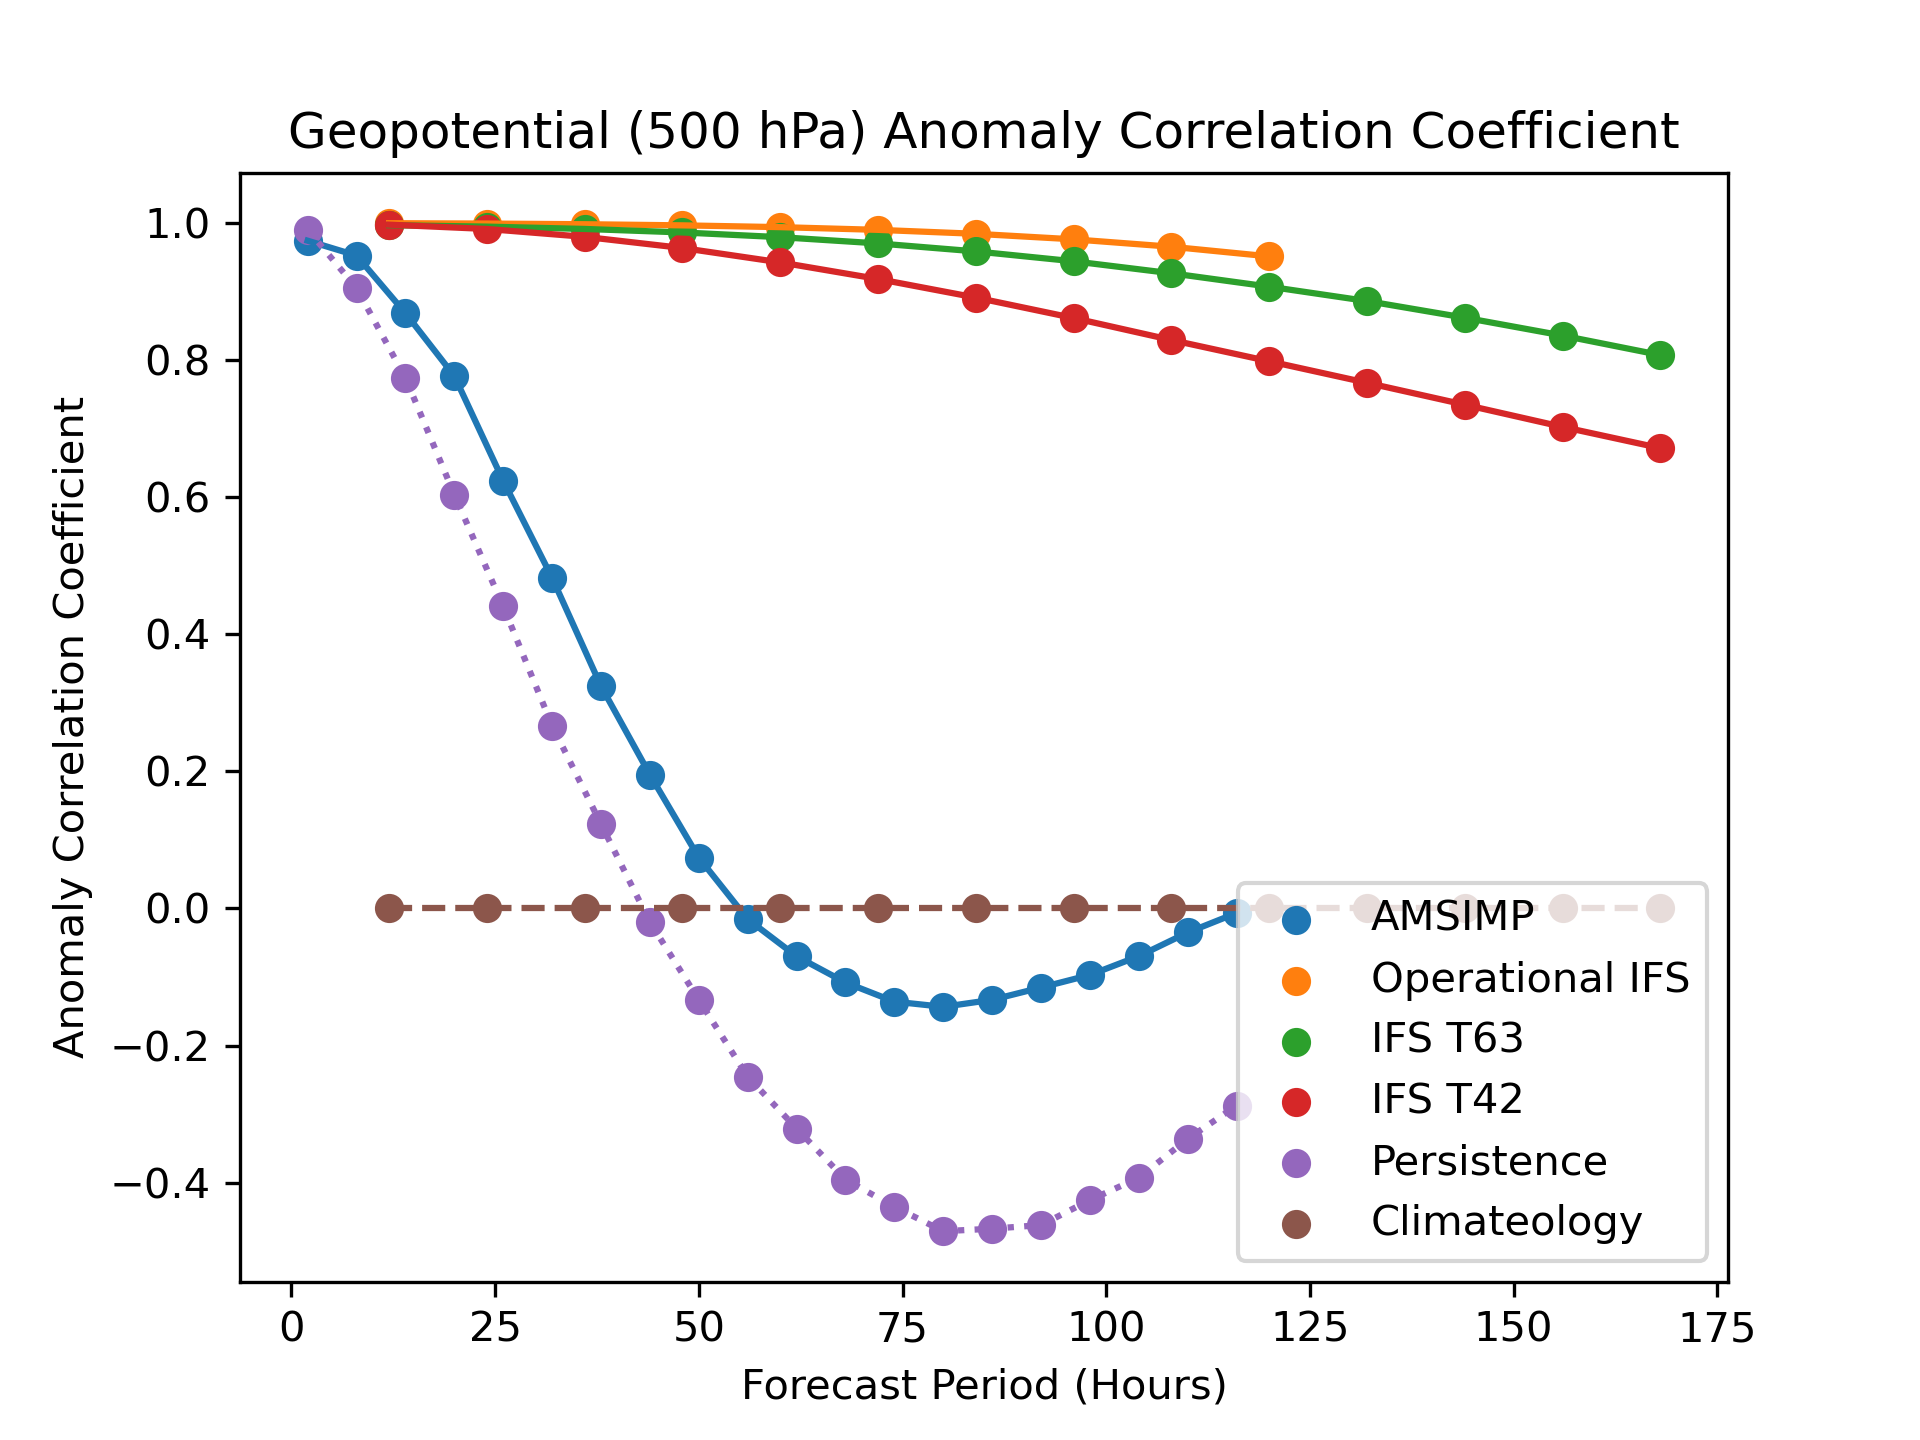
\includegraphics[width=.7\linewidth]{Plots/Results/Geopotential/anomaly_correlation_coefficient.png}
    \caption{Geopotential at 500 hPa}
\end{figure}
